Pour minimiser la moyenne sur la bande, on retient le mur plan en laine de verre, avec 38 points garnis sur 128. Son coût moyen vaut $0,627376$ et son maximum échantillonné $9,126397$. Si l'objectif prioritaire est de réduire le maximum, le mur plan en mélamine donne $7,270847$, avec une moyenne $0,679267$. Le critère de choix doit donc être annoncé.

La figure~\ref{fig:retenu} compare le placement retenu à un placement initial binaire de même quantité et à la paroi entièrement garnie. \code{evaluate_selected_configuration} reconstruit ce contrôle à partir des données du candidat. La moyenne initiale vaut $1,279166$ et le maximum initial $37,344859$, d'où des réductions respectives de $50,95\,\%$ et $75,56\,\%$. Ces gains comparent la même source, le même matériau, la même forme et le même nombre de points garnis.
\begin{figure}[!htbp]
\centering
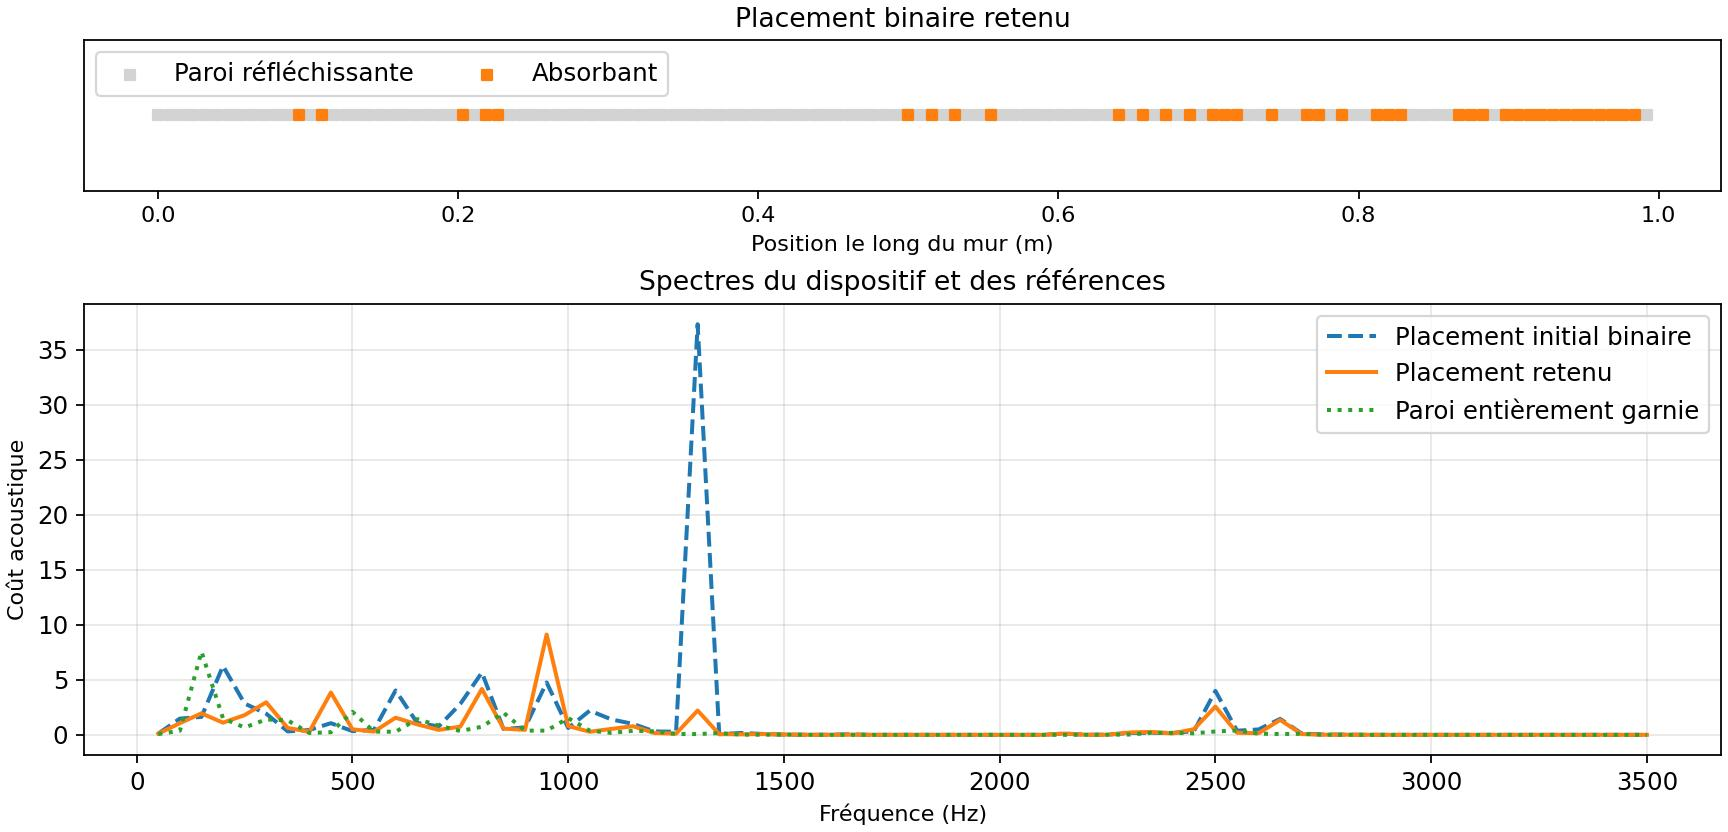
\includegraphics[width=.96\textwidth,height=.33\textheight,keepaspectratio]{resultats_comparaison_dispositifs/fig_dispositif_retenu.jpg}
\caption{Placement retenu et spectres des trois références de laine de verre}
\label{fig:retenu}
\end{figure}

La référence entièrement garnie a une moyenne $0,388505$. Le candidat utilise $70,31\,\%$ de points garnis en moins et son coût moyen est $61,48\,\%$ plus élevé que celui de cette référence. Il représente donc un compromis à budget réduit, avec un gain établi par rapport au placement initial de même quantité.
